\section{Durchführung}
\label{sec:Durchführung}

\subsection{Energieverteilung der beschleunigten Elektronen}
Der Versuch wird wie in \ref{fig:Aufbau} aufgebaut.
Dann wird der XY-Schreiber so kalibriert, dass die Breite des zu beschreibenden Blattes einem Bereich von 0 bis 10 Volt der Bremsspannung entspricht.
Es wird für eine Temperatur von ungefähr $\qty{25}{\celsius}$ der Auffängerstrom abhängig von der Bremsspannung $U_A$ aufgezeichnet.
Die Beschleunigungsspannung beträgt dabei $\qty{11}{\volt}$. 
Diese Messung wird noch einmal mit einer Temperatur von ungefähr $\qty{150}{\celsius}$ durchgeführt.


\begin{figure}[H]
    \centering
    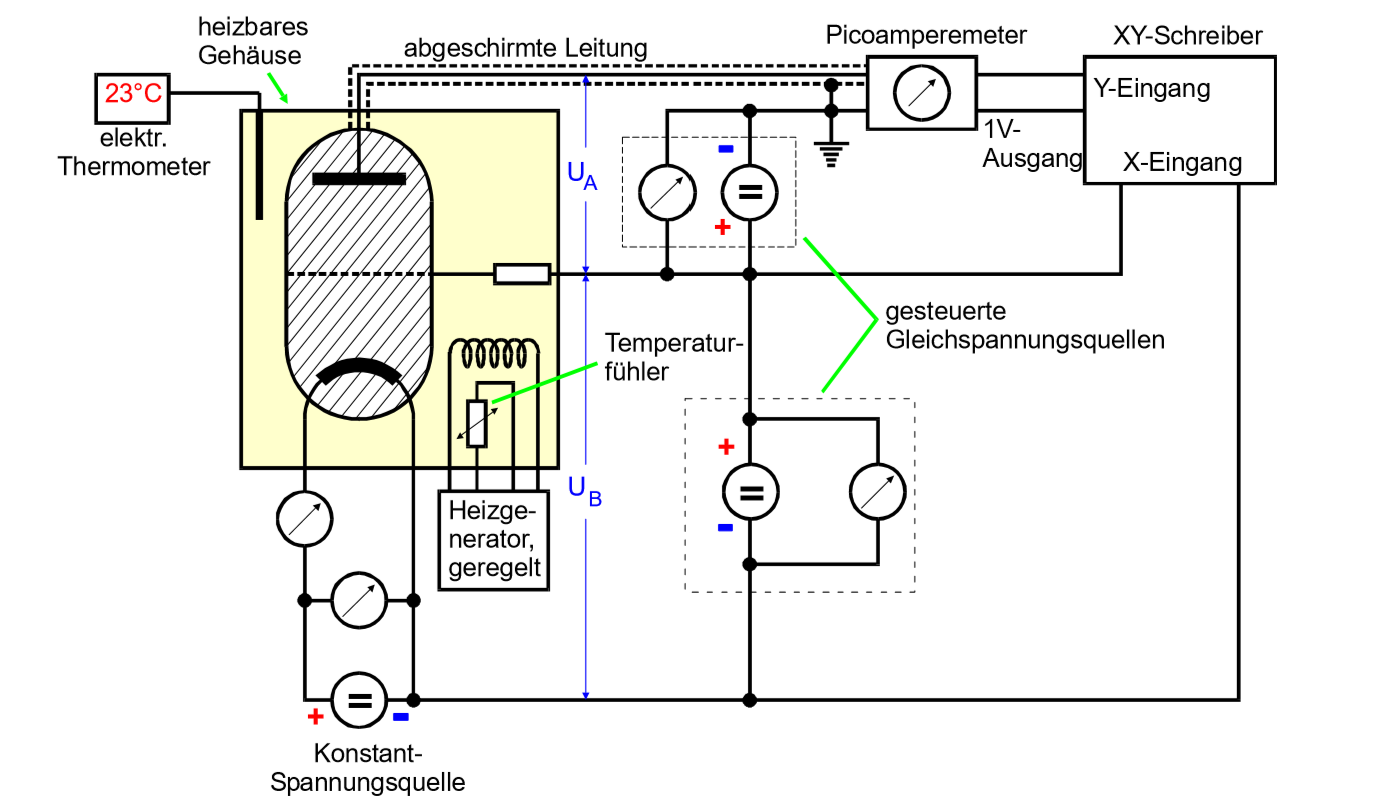
\includegraphics[width=\textwidth]{Bilder/Aufbau.png}
    \caption{Abgebildet ist der schmatische Aufbau des Franck-Hertz Versuches.}
    \label{fig:Aufbau}
\end{figure}

\subsection{Frank-Hertz-Kurve}
Um eine Frank-Hertz-Kurve zu messen wird der Auffängerstrom mithilfe des XY_Schreibers abhängig von der Beschleunigungsspannung aufgetragen.
Dies wird für drei Temperaturen zwischen $\qty{160}{\celsius}-\qty{200}{\celsius}$ für $\qty{0}{\volt}<U_B<\qty{60}{\volt}$ durchgeführt.